% Compile with the ACL Anthology LaTeX bundle on TeX path.
% pdflatex atrac3.tex && bibtex atrac3 && pdflatex atrac3.tex && pdflatex atrac3.tex
\documentclass[11pt]{article}

\usepackage[T1]{fontenc}
\usepackage[utf8]{inputenc}
\usepackage{microtype}
\usepackage{inconsolata}

% ACL house style. Use the [review] option if you want line numbers.
\usepackage{acl}

\usepackage{amsmath}
\usepackage{amssymb}
\usepackage{booktabs}
\usepackage{graphicx}
\usepackage{listings}
\usepackage{xcolor}
\usepackage{url}

\lstset{
  basicstyle=\ttfamily\footnotesize,
  breaklines=true,
  columns=fullflexible,
  keepspaces=true,
  showstringspaces=false,
  frame=single,
  framesep=3pt,
  rulecolor=\color{black!20},
  xleftmargin=4pt,
  xrightmargin=4pt,
}

\title{Revisiting the ATRAC3 Codec}

\author{Sangwhan Moon \\
  \texttt{sangwhan@iki.fi}
}

\begin{document}
\maketitle

\begin{abstract}
\noindent
This note documents \texttt{at3rs}, a Rust workbench implementation of Sony's
\textsc{atrac3} perceptual audio codec. \textsc{atrac3} is a constrained-bitrate
transform codec designed for the MiniDisc Long Play and Sony Memory Stick
families of products, operating at \(132\)/\(105\)/\(66\,\text{kbps}\) on
\(44.1\,\text{kHz}\) stereo input. We describe the codec's theoretical
formulation---a four-band quadrature mirror filter (QMF) tree feeding per-band
Modified Discrete Cosine Transforms (MDCT), followed by block-floating
quantization with a perceptually-weighted bit allocation and Huffman-coded
mantissas---and map every stage to its corresponding implementation in the
current source tree. The aim is a self-contained reference: enough math to
recover the algorithm from first principles, and enough code citations to
locate the constants, tables, and decision rules used by the current encoder.
\end{abstract}

\noindent\footnotesize
ATRAC, ATRAC3, ATRAC3plus, ATRAC Advanced Lossless and their logos are
trademarks of Sony Corporation.
\normalsize

\section{Introduction}
\label{sec:intro}

\textsc{atrac3} (\textit{Adaptive TRansform Acoustic Coding 3}) is a
perceptual audio codec belonging to the same family as MPEG-1 Layer III, AAC,
and Dolby AC-3: a critically-sampled, transform-based coder that quantizes
spectral coefficients under a perceptual masking budget, then losslessly
packs the resulting bitstream. It was deployed by Sony in MiniDisc-LP, ATRAC
Audio Device (Walkman), and certain PlayStation Portable titles, and remains
the format of choice for several reverse-engineered legacy toolchains.

\texttt{at3rs} is a from-scratch Rust implementation of the encoding side of
\textsc{atrac3}. The current encoder emits RIFF/WAVE ATRAC3 files that are
accepted by Sony's PSP ATRAC tool; exact quality parity with Sony's encoder is
still an active target. The decoding path exists for matrix evaluation but is
not yet usable quality. The workbench is structured around a small number of
files:

\begin{lstlisting}[language=]
src/atrac3.rs   - filterbank, MDCT, gain/tonal experiments, BFU plan, packer
src/atrac3/     - channel state, constants, config, debug helpers
src/codec.rs    - codec-agnostic I/O glue
src/dsp.rs      - shared helpers
src/eval.rs     - SNR/PSNR roundtrip metrics
eval/           - local matrix evaluation runner
src/gha.rs      - tonal-analysis support types
src/huffman.rs  - canonical Huffman tables
src/psychoacoustic.rs - shared PA helpers
\end{lstlisting}

The remainder of this document follows the encode path top to bottom:
\S\ref{sec:pipeline} sketches the frame layout and pipeline,
\S\ref{sec:filterbank} derives the QMF/MDCT analysis,
\S\ref{sec:bfu} describes the block-floating spectral representation,
\S\ref{sec:bitalloc} details the perceptual bit allocator,
\S\ref{sec:entropy} covers entropy coding and bitstream packing, and
\S\ref{sec:status} discusses unfinished components, public-surface decisions,
and evaluation.

\section{Pipeline Overview}
\label{sec:pipeline}

\textsc{atrac3} operates on fixed-size frames of \(N{=}1024\) PCM samples per
channel at \(F_s{=}44{,}100\,\text{Hz}\), corresponding to a frame duration of
\(\approx 23.2\,\text{ms}\). The frame size is \emph{not} a free parameter: it
is baked into the QMF delay line, the MDCT length, and the bitstream
container format. The supported stream bitrates correspond to per-channel
byte budgets

\begin{equation}
    B_{\text{ch}} \in \{96,\; 152,\; 192\}\ \text{bytes/frame},
\end{equation}

\noindent
i.e.\ \(66\), \(105\), and \(132\,\text{kbps}\) for mono, doubled for stereo.
Selection logic lives in \texttt{choose\_atrac3\_block\_align} at
\texttt{src/encoder.rs}, which simply rounds the requested bitrate to the
nearest valid budget.

The encoder is a strict pipeline (\texttt{Atrac3Context::encode\_frame}):

\begin{enumerate}
\itemsep0pt
\item Convert interleaved \texttt{i16} PCM to planar \(f32\) in \([-1,1]\).
\item Per channel, run the two-level QMF analysis tree to produce four
\(256\)-sample subbands.
\item Per subband, run a length-\(512\) MDCT (with \(256\)-sample overlap)
to obtain \(256\) spectral coefficients per band, for \(1024\) coefficients
total per channel.
\item Optionally detect gain-control points and experimental tonal
components. These paths are controlled by explicit \texttt{EncoderConfig}
fields and CLI flags, and are disabled by default.
\item Group the residual \(1024\) coefficients into \(32\) Block Floating
Units (BFUs); for each BFU, choose a quantizer selector
\(s \in \{0,\dots,7\}\) and a scale-factor index \(k \in \{0,\dots,63\}\).
\item Iterate the selector assignment under a perceptually-weighted budget
search, then run shaping/refinement passes until the total bit count fits the
per-channel budget \(B_{\text{ch}}\).
\item Pack the BFU header, scale-factor indices, and quantized mantissas
into the per-channel sound unit, choosing between Huffman (\textsc{vlc}) and
fixed-length (\textsc{clc}) mantissa coding on a frame-global basis.
\end{enumerate}

The command-line tool also exposes an experimental \texttt{-d} path so the
evaluation matrix can exercise \texttt{decode\_frame}. That decoder is known
to be poor quality today and is diagnostic only; it is not a supported
listening-quality decoder.

\section{Filterbank: QMF Tree and MDCT}
\label{sec:filterbank}

\subsection{Two-stage QMF analysis}

\textsc{atrac3} uses a Polyphase Quadrature Filterbank (PQF) tree that
splits the input into four contiguous, equal-bandwidth subbands. The
prototype filter is a \(48\)-tap symmetric FIR encoded as a \(24\)-tap half
filter at \texttt{src/atrac3.rs:16}, expanded in
\texttt{QMF\_WINDOW} (\texttt{src/atrac3.rs:25}) by mirroring and a factor-of-two
gain compensation:

\begin{equation}
    h[n] = h[47-n] = 2\,h_{\text{half}}[n],\quad n=0,\dots,23.
\end{equation}

Let \(x[n]\) be the input. A single QMF stage produces low- and high-pass
half-rate outputs

\begin{align}
y_{\ell}[m] &= \sum_{i=0}^{23}\!\Big(h[2i]\,x[2m{+}47{-}2i] \nonumber \\
            &\hphantom{= \sum_{i=0}^{23}\!\Big(} + h[2i{+}1]\,x[2m{+}46{-}2i]\Big), \label{eq:qmf_lo}\\
y_{h}[m]    &= \sum_{i=0}^{23}\!\Big(h[2i]\,x[2m{+}47{-}2i] \nonumber \\
            &\hphantom{= \sum_{i=0}^{23}\!\Big(} - h[2i{+}1]\,x[2m{+}46{-}2i]\Big), \label{eq:qmf_hi}
\end{align}

\noindent
i.e., a polyphase decomposition of the prototype \(h\) where the high-band is
formed by alternating-sign modulation of the odd-indexed taps. The
implementation lives in \texttt{pqf\_forward} at
\texttt{src/atrac3.rs:1633} and maintains a \(46\)-sample history per stage in
\texttt{Atrac3ChannelUnit::an\_delay\_buf\{1,2,3\}}.

The full analysis applies three stages organised as a tree
(\texttt{analyze\_frame}, \texttt{src/atrac3.rs:480}):

\begin{enumerate}
\itemsep0pt
\item Stage~1: \(1024\!\to\!\)~\(512\,\text{lo} \mathbin{\Vert} 512\,\text{hi}\).
\item Stage~2a: \(512\,\text{lo}\!\to\!256\,\text{B}_0 \mathbin{\Vert} 256\,\text{B}_1\).
\item Stage~2b: \(512\,\text{hi}\!\to\!256\,\text{B}_3 \mathbin{\Vert} 256\,\text{B}_2\).
\end{enumerate}

\noindent
Note that the second split of the high band yields the four output bands in
the order \(\text{B}_0, \text{B}_1, \text{B}_2, \text{B}_3\) once
\(\text{B}_2\) and \(\text{B}_3\) are swapped: the inner high-band split's
own high-pass output corresponds to band \(\text{B}_3\), the highest
frequency. This swap is applied unconditionally in
\texttt{analyze\_frame}. At \(F_s = 44.1\,\text{kHz}\) the four bands cover
\([0,\,5.5125]\), \([5.5125,\,11.025]\), \([11.025,\,16.5375]\), and
\([16.5375,\,22.05]\,\text{kHz}\).

\subsection{Per-band MDCT}

Each \(256\)-sample subband is then transformed by a length-\(2N\), \(N{=}256\)
MDCT with \(50\%\) overlap. Recall that the analysis MDCT is

\begin{equation}
    X[k] = \!\!\sum_{n=0}^{2N-1}\!\! w_a[n]\,x[n]\cos\!\Big(\tfrac{\pi}{N}(n{+}\tfrac{N{+}1}{2})(k{+}\tfrac{1}{2})\Big),
\end{equation}

\noindent
for \(k = 0,\dots,N-1\), with the standard time-domain aliasing cancellation
(TDAC) constraint \(w_a[n]\,w_s[n] + w_a[n{+}N]\,w_s[n{+}N] = 1\) for the
overlap-add to recover the original samples after inverse MDCT.

\paragraph{Window choice.}
\textsc{atrac3} uses an asymmetric design where the analysis window
\(w_a\) is the lifted half-sine

\begin{equation}
    w_a[n] = 1 + \sin\!\Big((\tfrac{n+0.5}{256} - 0.5)\,\pi\Big), \quad n=0,\dots,255,
    \label{eq:enc_window}
\end{equation}

\noindent
encoded directly in \texttt{ENCODE\_WINDOW}
(\texttt{src/atrac3.rs:54}). The synthesis window is derived from
\(w_a\) via the canonical Princen--Bradley dual

\begin{equation}
    w_s[n] = \frac{2\,w_a[n]}{w_a[n]^2 + w_a[255-n]^2},
    \label{eq:dec_window}
\end{equation}

\noindent
which is precomputed as \texttt{DECODE\_WINDOW}
(\texttt{src/atrac3.rs:62}) and ensures TDAC perfect reconstruction. The
auxiliary half-sine \texttt{MDCT\_WINDOW} (\texttt{src/atrac3.rs:44}) is
used only by the FFT-based MDCT kernel below.

\paragraph{Fast MDCT via FFT-128.}
The implementation factors the length-\(512\) MDCT through a length-\(N/4 =
128\) complex FFT (provided by \texttt{rustfft}). The standard derivation
is to fold \(2N\) reals into \(N/2\) complex samples using the symmetry of
the cosine basis. \texttt{at3rs} computes pre- and post-twiddle tables

\begin{align}
\alpha &= \frac{2\pi}{8\cdot 2N}, \quad \omega = \frac{2\pi}{2N}, \\
c_i &= s_{\text{scale}}\cos(\omega i + \alpha),\\
s_i &= s_{\text{scale}}\sin(\omega i + \alpha),
\end{align}

\noindent
with \(s_{\text{scale}} = \sqrt{1/(2N)}\) for the forward direction
(\texttt{src/atrac3.rs:344}) and \(s_{\text{scale}} = \sqrt{N/(2N)} \cdot
\sqrt{2}\) effectively for the inverse. The pre-twiddle folds the input as

\begin{align}
r_0 &= x[3N/2 - 1 - i] + x[3N/2 + i], \\
i_0 &= x[N/2 + i] - x[N/2 - 1 - i], \\
Z[i/2] &= (r_0 c_i + i_0 s_i,\ i_0 c_i - r_0 s_i),
\end{align}

\noindent
for \(i \in [0, N/2)\) (\texttt{src/atrac3.rs:358}), with the symmetric
re-folding for \(i \in [N/2, N)\). After the FFT the post-twiddle stores
\(\,X[2j] = -r_j c_j - i_j s_j\,\) and \(\,X[N-1-2j] = -r_j s_j + i_j c_j\,\)
(\texttt{src/atrac3.rs:376}).

\paragraph{Odd-band reversal.}
Bands \(\text{B}_1\) and \(\text{B}_3\) are spectrally reversed prior to or
after their MDCT (\texttt{odd\_band == true},
\texttt{src/atrac3.rs:389}). This compensates for the alternating sign
introduced by each polyphase QMF stage so that the concatenated
\(4\!\times\!256 = 1024\)-bin spectrum has a monotonic frequency mapping
when reassembled.

\section{Spectral Grouping and Block-Floating Quantization}
\label{sec:bfu}

\subsection{Block Floating Units}

The \(1024\) MDCT coefficients are partitioned into \(32\) non-uniform
\emph{Block Floating Units} (BFUs) defined by the boundary table
\texttt{ATRAC3\_SUBBAND\_TAB} at \texttt{src/atrac3.rs:99}:

\begin{small}
\[
[0, 8, 16, 24, 32, 40, 48, 56,\,
   64, 80, 96, 112, 128, 144, 160, 176,
\]
\[
   192, 224, 256, 288, 320, 352, 384, 416,\,
   448, 480, 512, 576, 640, 704, 768, 896, 1024].
\]
\end{small}

\noindent
The widths grow approximately geometrically with frequency, mimicking the
critical-band structure of human hearing: \(8\)-bin BFUs in the lowest
\(\sim\!350\,\text{Hz}\), \(128\)-bin BFUs in the highest \(\sim\!5\,\text{kHz}\).

Within each BFU \(b\) of width \(L_b\), the spectral block
\(\mathbf{X}_b = (X[i])_{i \in [\text{start}_b,\text{end}_b)}\) is encoded as a
single shared scale factor \(\sigma_b\) (the \emph{block float exponent}) and
\(L_b\) signed mantissas \(\mathbf{q}_b\):

\begin{equation}
    \widehat{X}[i] = q[i]\,\frac{\sigma_b}{Q_s},
\end{equation}

\noindent
where \(Q_s\) is the per-selector quantizer maximum (Table~\ref{tab:selectors}).

\subsection{Scale-factor table}

The scale-factor codebook contains \(64\) values logarithmically spaced
\(\tfrac{1}{3}\) bit apart:

\begin{equation}
    \sigma[k] = 2^{k/3 - 21},\qquad k = 0,\dots,63,
\end{equation}

\noindent
implemented in the ATRAC3 constant table. The minimum representable level is
\(2^{-21}\!\approx\!4.8\!\cdot\!10^{-7}\) and the maximum is
\(2^{42/3}\!\approx\!100.3\). Each BFU uses a \(6\)-bit field to transmit \(k\).

\subsection{Quantizer selectors}

A BFU's bit budget is determined by its \emph{selector} \(s_b \in \{0,\dots,7\}\),
where \(s_b = 0\) means the entire BFU is treated as zero (no mantissas
transmitted, no scale factor transmitted). The non-zero selectors define
quantizer maxima

\begin{table}[ht]
\centering\small
\begin{tabular}{cccc}
\toprule
\(s\) & \(Q_s\) & \(|q|_{\max}\) & nominal bits/coeff \\
\midrule
1 & 1.5  &  1 & \(\sim\!2\) (paired) \\
2 & 2.5  &  2 & 3 \\
3 & 3.5  &  3 & 3 \\
4 & 4.5  &  4 & 4 \\
5 & 7.5  &  7 & 4 \\
6 & 15.5 & 15 & 5 \\
7 & 31.5 & 31 & 6 \\
\bottomrule
\end{tabular}
\caption{Per-selector quantizer parameters used by the BFU planner.}
\label{tab:selectors}
\end{table}

For a BFU with chosen \(\sigma_b\) and \(s_b\), each coefficient is encoded
as

\begin{equation}
    q[i] = \mathrm{clip}\!\left(\mathrm{round}\!\left(\frac{X[i]}{\sigma_b}\,Q_{s_b}\right),\,-|q|_{\max},\,|q|_{\max}\right).
    \label{eq:quant}
\end{equation}

\subsection{Energy-preserving rounding}

A naive midpoint round to nearest minimises per-coefficient \(L^2\) error
but biases the per-block reconstructed energy: dense small-magnitude
coefficients tend to round to \(0\), reducing total spectral power and
producing audibly hollow textures. \texttt{quantize\_block\_energy\_adjusted}
addresses this by collecting \emph{borderline} coefficients, those whose
unrounded value lies near a half-integer, and iteratively flipping their
rounding direction toward whichever choice (up or down by one quantum) brings
reconstructed block energy closer to \(\sum_i X[i]^2\). The candidate list is
sorted by how close each value is to the half-integer boundary so that the
cheapest swaps are applied first. The result is a quantizer that is no longer
strictly minimum-MSE but preserves block-level loudness. This energy-adjusted
rounding is the default; \texttt{AT3RS\_DISABLE\_SF\_SEARCH} and related
configuration flags can disable some of the surrounding search machinery for
experiments.

\section{Perceptually-Weighted Bit Allocation}
\label{sec:bitalloc}

The encoder must choose \((s_b, k_b)_{b=0}^{31}\) for each channel under the
constraint that the total emitted bits do not exceed \(8\,B_{\text{ch}}\). At
the high end of the allowed bitrate (\(132\,\text{kbps}\)) the allocator can
afford a near-uniform selector pattern; at \(66\,\text{kbps}\) it is forced
into aggressive masking decisions.

\subsection{Loudness and absolute threshold of hearing}

The first ingredient is the \emph{equal-loudness curve}
\(\mathcal{L}[i]\), a \(1024\)-bin weighting precomputed at
\texttt{src/atrac3.rs:72} as

\begin{align}
f_i &= \frac{(i+3)\cdot F_s/2}{1024}, \\
t_i &= -10(\log_{10} f_i - 3.5)^2 + 3 - \frac{f_i}{3000}, \\
\mathcal{L}[i] &= 10^{0.1\, t_i}.
\end{align}

\noindent
This is a smooth quadratic-in-log frequency bowl peaked near \(3\,\text{kHz}\)
with a high-frequency rolloff, used to weight per-bin energy when computing
the channel loudness norm \(\Lambda_{\text{ch}}\) below.

The second ingredient is the per-BFU \emph{absolute threshold of hearing}
(ATH), \(T_{\text{ATH}}[b]\). The Frank approximation
\texttt{ath\_formula\_frank} (\texttt{src/atrac3.rs:124}) provides per-bin
SPL thresholds via a \(140\)-entry tabulated curve indexed in
\(\log_{10}(f/100)\) with frac-linear interpolation:

\begin{align}
\ell &= 40\log_{10}(f/100), \\
\text{ATH}_{\text{dB}}(f) &= \mathrm{TAB}[\lfloor\ell\rfloor]\,(1{-}\{\ell\}) + \mathrm{TAB}[\lfloor\ell\rfloor+1]\{\ell\}.
\end{align}

\noindent
After subtracting the \(100\,\text{dB}\) calibration offset and the
\(0.015\,(\,f/1\,\text{kHz})^2\) high-frequency tilt
(\texttt{calc\_ath\_spec}, \texttt{src/atrac3.rs:147}), the minimum threshold
inside each BFU is converted back to linear amplitude and stored in
\texttt{ATRAC3\_ATH\_BFU} (\texttt{src/atrac3.rs:83}).

The current implementation does \emph{not} compute simultaneous (in-band) or
non-simultaneous (temporal) masking thresholds. The masking model is the
absolute threshold scaled by a tracked global loudness, described next.

\subsection{Tracked loudness norm}

Per-frame loudness in channel \(c\) is

\begin{equation}
    L_c = \sum_{i=0}^{1023} X_c[i]^2 \,\mathcal{L}[i],
\end{equation}

\noindent
(\texttt{frame\_channel\_loudness}, \texttt{src/atrac3.rs:819}). A first-order
exponential filter tracks the global loudness across frames:

\begin{equation}
    \Lambda_t = 0.98\,\Lambda_{t-1} + 0.01 \sum_c L_{c,t},
\end{equation}

\noindent
and the masking threshold for BFU \(b\) becomes

\begin{equation}
    T_b = T_{\text{ATH}}[b] \cdot \frac{\Lambda_t}{\Lambda_{\text{factor}}},
    \quad \Lambda_{\text{factor}} = 0.006.
    \label{eq:masking}
\end{equation}

\noindent
A BFU whose energy falls below \(T_b\) is forced to selector \(0\) and the
mantissas/scale factor are not coded. The constants \(0.98\), \(0.01\), and
\(\Lambda_{\text{factor}}\) (\texttt{src/atrac3.rs:122}) were tuned
empirically on the payload fixtures in \texttt{fixtures/}.

\subsection{Per-BFU importance score}

Each BFU is assigned a scalar importance combining bulk energy with peak
prominence:

\begin{equation}
    I_b = \big(\sqrt{E_b} + 8\,M_b\big) \cdot \big(1 + 0.2\,\phi_b\big) \cdot \big(1 + 0.05\,\beta_b\big),
    \label{eq:importance}
\end{equation}

\noindent
where \(E_b = \sum_{i \in b} X[i]^2\), \(M_b = \max_i |X[i]|\), \(\phi_b\) is
the entry of \texttt{ATRAC3\_FIXED\_ALLOC\_TABLE} for BFU \(b\)
(\texttt{src/atrac3.rs:107}), and \(\beta_b \in \{0,1,2,3\}\) is the QMF band
index. The peak weighting \(8 M_b\) biases the allocator toward preserving
tonal/transient peaks even when bulk energy is small.

\subsection{Initial selector heuristic}

A scale-factor variance term \(\rho_b\) measures how broadband-flat the
block is:

\begin{equation}
    \rho_b = \min\!\Big(\sqrt{\mathrm{Var}(k_b)},\ 14\Big)\,/\,14,
\end{equation}

\noindent
ranging from \(0\) (all coefficients near the same magnitude) to \(1\)
(highly heterogeneous). The initial selector is then computed as

\begin{equation}
    s_b = \mathrm{clip}\!\left(\Big\lfloor \rho_b \tfrac{k_b}{D_b} + (1{-}\rho_b)\,\phi_b - \delta + \gamma_b \Big\rfloor,\;0,\;7\right),
    \label{eq:initial_selector}
\end{equation}

\noindent
where \(D_b\) is a block-dependent divisor
(\texttt{selector\_spread\_divisor}, \texttt{src/atrac3.rs:686}) ranging
from \(2.6\) at low frequency to \(6.0\) at high frequency, \(\delta\) is a
global shift parameter swept during the budget search, and \(\gamma_b\)
bundles three additional perceptual biases:

\begin{itemize}
\itemsep0pt
\item \(\gamma_b^{(I)}\), an \emph{importance boost} from
Eq.~\ref{eq:importance} stepping over the thresholds \(\{3.5, 6.0, 10.0\}\)
to \(\{0, 0.5, 1.0, 2.0\}\) (\texttt{importance\_boost},
\texttt{src/atrac3.rs:665}),
\item \(\gamma_b^{(M)}\), an \emph{average magnitude bias} based on
\(\log_{10} \overline{|X|_b}\) (\texttt{avg\_mag\_bias},
\texttt{src/atrac3.rs:649}), giving negative \(\gamma\) for very quiet
blocks and positive for very loud ones,
\item \(\gamma_b^{(S)}\), a \emph{shape hint}
(\texttt{ATRAC3\_SELECTOR\_SHAPE\_HINT}, \texttt{src/atrac3.rs:113}) decaying
from \(7\) in the lowest BFUs to \(0\) at the top, encoding the prior that
high frequencies generally tolerate coarser quantization.
\end{itemize}

\noindent
The clip is special-cased so a non-zero \(s_b\) is never mapped to \(0\)
implicitly --- selector \(0\) only happens through the explicit masking
check of Eq.~\ref{eq:masking}.

\subsection{Budget search and refinement}

The current planner performs a binary search over a global selector shift
\(\delta \in [-8,20]\), recomputing the full \(32\)-BFU plan for each trial
and retaining the best plan whose encoded bit count does not exceed the
per-channel budget. Before the search, the effective budget is reduced by
header overhead for gain/tonal side data and, when VLC is enabled, by a small
configurable safety margin (\texttt{EncoderConfig::vlc\_bit\_safety}, default
\(32\) bits). This keeps later coding-mode decisions from accidentally
overflowing the sound-unit payload.

Once the binary search chooses a feasible plan, the encoder runs a sequence
of shaping passes. The default pass, \texttt{fit\_bfu\_plan\_to\_budget},
tries local selector changes and accepts changes that improve weighted
reconstruction error while remaining under budget. Additional experimental
passes can be enabled from \texttt{EncoderConfig}:

\begin{itemize}
\itemsep0pt
\item \texttt{enable\_tail\_prune}: enforce a non-increasing
high-frequency selector tail.
\item \texttt{experimental\_concentrate\_bits}: prune low-energy
high-frequency BFUs when they only receive very low precision.
\item \texttt{experimental\_tonal\_prune}: preserve a small set of
dominant BFUs on concentrated tonal frames and prune weaker neighbours.
\item \texttt{enable\_tail\_sf\_smooth}: smooth tail scale-factor
indices to avoid abrupt high-frequency gain jumps.
\item \texttt{disable\_reference\_shape}: opt out of the default pass
that nudges selectors toward the reference-shaped high-frequency allocation
prior.
\item \texttt{experimental\_rebalance\_bfus}: try donor/receiver
precision swaps and keep a candidate if weighted error improves.
\item \texttt{cap\_high\_bfus}: clear BFUs above a fixed high-frequency
cutoff for debugging.
\end{itemize}

\noindent
After every shaping pass, the planner recomputes the channel coding mode and
re-runs budget fitting. This makes the allocation stage a small
rate--distortion search rather than a single feed-forward selector formula.

\section{Entropy Coding and Bitstream}
\label{sec:entropy}

\subsection{Coding mode}

Mantissas are emitted in one of two modes, signaled by a single bit:

\begin{itemize}
\itemsep0pt
\item \textsc{vlc} (\texttt{coding\_mode = 0}): canonical Huffman codes,
selector-dependent, with selector \(1\) using a paired-symbol alphabet over
\((q_a, q_b)\) so that highly-quantized blocks (where most coefficients are
\(0, \pm 1\)) get sub-bit-per-coefficient rates.
\item \textsc{clc} (\texttt{coding\_mode = 1}): fixed-length two's-complement
codes at the nominal width of Table~\ref{tab:selectors}.
\end{itemize}

The selection is made per channel by
\texttt{channel\_prefers\_vlc}. VLC is disabled when
\texttt{EncoderConfig::force\_clc} or \texttt{EncoderConfig::disable\_vlc} is set. Otherwise
the encoder optionally rejects plans whose non-zero selectors exceed
\texttt{EncoderConfig::vlc\_max\_selector}; for the remaining plans it chooses VLC
whenever the summed spectral VLC bit count is lower than the summed CLC bit
count. The global budget search already subtracts the configurable VLC safety
margin described above, so the mode decision itself is a direct CLC-versus-VLC
bit-count comparison.

\subsection{Huffman tables}

The seven Huffman codebooks (one per non-zero selector) are stored as
\((\text{symbol},\,\text{length})\) pairs in
\texttt{ATRAC3\_HUFFTABS\_RAW} (\texttt{src/huffman.rs:131}). The encoder
materialises them into a canonical form
(\texttt{src/huffman.rs:77}) that assigns codes by ascending
\((\text{length},\,\text{symbol})\) order, matching the FFmpeg reference.
Symbols for selectors \(2\)--\(7\) are derived from a signed magnitude via

\begin{equation}
    \text{sym}(q) = \begin{cases}
        2|q|       & q \geq 0 \\
        2|q| + 1   & q < 0
    \end{cases}\;-\;1,
    \label{eq:scalar_vlc}
\end{equation}

\noindent
(\texttt{scalar\_vlc\_symbol}, \texttt{src/atrac3.rs:1414}). Selector \(1\)
maps the \(9\) possible \((q_a,q_b) \in \{-1,0,+1\}^2\) pairs to a
\(0\)--\(8\) alphabet directly (\texttt{selector1\_vlc\_symbol},
\texttt{src/atrac3.rs:1308}).

\subsection{Per-channel sound unit layout}

Each channel's sound unit is laid out as (\texttt{write\_channel\_sound\_unit},
\texttt{src/atrac3.rs:1336}):

\begin{lstlisting}[language=]
[ 6 b ] sync prefix      = 0x28
[ 2 b ] frame_type       = 3
[12 b ] reserved
[ 5 b ] joint_stereo_info= 0
[ 5 b ] num_blocks - 1
[ 1 b ] coding_mode      (0=VLC, 1=CLC)
[ 3 b ] selector[0..num_blocks]   each
[ 6 b ] sf_idx[0..num_blocks]     for nonzero sel.
[ var ] mantissas (VLC or CLC)
[ pad ] zero-fill to channel budget
\end{lstlisting}

\noindent
Streams are wrapped in a RIFF/WAVE container with format tag
\(0\text{x}0270\) (ATRAC3) and a \texttt{fact} chunk advertising the per-channel
sample count and the \(1024\) samples-per-frame value
(\texttt{write\_at3\_riff}, \texttt{src/main.rs:244}). An optional
\texttt{smpl} chunk carries loop points for streams used in interactive
applications.

\section{Joint Stereo, Gain/Tonal Coding, and Evaluation}
\label{sec:status}

\subsection{Joint stereo (not implemented)}

The reference \textsc{atrac3} bitstream supports a joint-stereo mode
(intensity-coded high frequencies above a per-frame split point with a
single transmitted scale per coupled BFU). \texttt{at3rs} reserves the
\texttt{joint\_stereo\_info} field but always transmits \(0\), encoding
each channel independently. This is consistent with the FFmpeg decoder
behaviour for \texttt{joint\_stereo\_info == 0} but represents a hard
ceiling on stereo bitrate efficiency: a true joint-stereo path could save
\(\sim\!20\%\) of the high-frequency bit budget on correlated material.

\subsection{Gain control and tonal coding}

ATRAC3 sound units can carry gain-control side data and tonal components in
addition to the residual MDCT spectrum. \texttt{at3rs} now contains
experimental implementations for both, but they are deliberately disabled in
the default encoder configuration because neither path is yet a quality win
on the fixture corpus.

Gain detection is enabled with \texttt{EncoderConfig::experimental\_gain} or the
newer \texttt{EncoderConfig::experimental\_gain\_v2}; the CLI exposes the v2
path as \texttt{--enable-gain-v2}. The encoder searches each QMF
band for short-time energy changes and writes gain points before MDCT
packing. When gain points are present, the corresponding side-information
bits are subtracted from the BFU budget and the analysis windows are modulated
so that the residual spectrum matches the transmitted gain envelope.

Tonal components are enabled with
\texttt{EncoderConfig::experimental\_tonal\_components}; the CLI exposes this
as \texttt{--enable-tonal-components}. The detector looks for
locally dominant spectral peaks, quantizes short runs with high precision
(selector \(7\)), groups compatible components, writes them in the tonal
substream, and subtracts their reconstructed contribution from the residual
before BFU planning. Separately, the default planner includes a
\emph{tonal-frame boost}: if energy is concentrated in a few BFUs, the
planning spectrum is temporarily boosted and the written scale factors are
offset back down. This is not the same as emitting tonal syntax; it is a
bit-allocation heuristic for exposed tonal material.

\subsection{Evaluation}

\texttt{src/eval.rs} provides \texttt{evaluate\_pair}, an offset-search
quality scorer used by the Rust test harness. Given an original PCM signal
\(x\) and a reconstructed signal \(\hat x\), the function searches an
offset window \([0, W]\) (default \(W = 4096\)) and reports

\begin{align}
\text{SNR}_\text{dB}(\tau) &= 10\log_{10}\!\frac{\sum x[n]^2}{\sum (x[n] - \hat x[n+\tau])^2}, \\
\text{PSNR}_\text{dB}(\tau) &= 20\log_{10}\!\frac{32767}{\text{RMSE}(\tau)},
\end{align}

\noindent
selecting the \(\tau^\star\) maximising SNR. This compensates for the
frame-aligned encoding/decoding delay introduced by the QMF and MDCT
stages without a separate \emph{a priori} delay estimate. \texttt{tests/quality.rs}
and \texttt{tests/payload\_quality.rs} use the metric to gate regressions
on the fixture corpus in \texttt{fixtures/}.

For local listening and cross-implementation debugging, the primary workflow
is now \texttt{eval/run\_eval.py}. It evaluates an encoder/decoder comparison
matrix for each fixture:

\begin{center}
\begin{tabular}{cc}
\toprule
encoder & decoder \\
\midrule
\texttt{at3rs} & \texttt{at3rs} \\
\texttt{at3rs} & Sony \texttt{psp\_at3tool.exe} \\
Sony \texttt{psp\_at3tool.exe} & \texttt{at3rs} \\
Sony \texttt{psp\_at3tool.exe} & Sony \texttt{psp\_at3tool.exe} \\
\bottomrule
\end{tabular}
\end{center}

\noindent
The script writes decoded WAVs, a CSV summary, and a self-contained HTML
report with base64-inlined metric plots under
\texttt{output/<git-ref>/eval/<input-dir>/}. It can also run ViSQOL and PEAQ
when the third-party binaries are present. This matrix is intentionally
diagnostic: \texttt{at3rs->sony} measures the current encoder through Sony's
decoder, \texttt{sony->sony} is the local reference loop, and any cell ending
in \texttt{at3rs} tracks the known-broken at3rs decoder.

Figures~\ref{fig:current-snr}--\ref{fig:current-peaq} show the most recent
full-fixture matrix available at the time of writing, measured on
2026-04-30 from
\texttt{output/main@6775023-dirty/eval/fixtures/summary.csv}. These plots are
intended as a dated snapshot, not a permanent benchmark: the output directory
is keyed by git ref so future runs can be compared against the exact source
revision that produced them.

\begin{figure}[t]
\centering
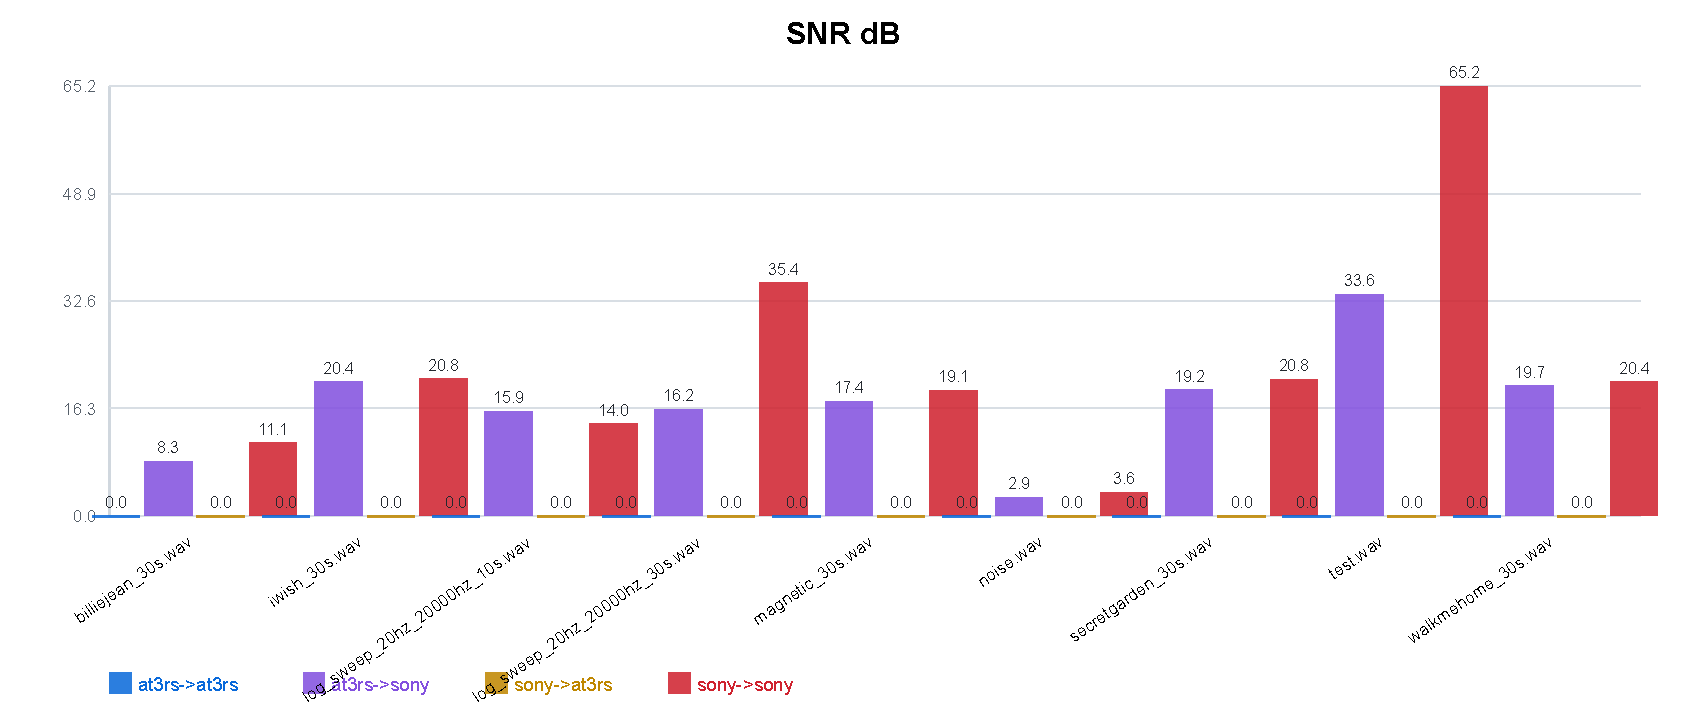
\includegraphics[width=\linewidth]{figures/current_snr_db.pdf}
\caption{Current round-trip SNR by fixture and encoder/decoder cell. The
\texttt{at3rs->sony} cell measures the at3rs encoder through Sony's decoder,
while \texttt{sony->sony} is the local Sony-tool reference loop; cells decoded
by \texttt{at3rs} expose decoder work still to be done.}
\label{fig:current-snr}
\end{figure}

\begin{figure}[t]
\centering
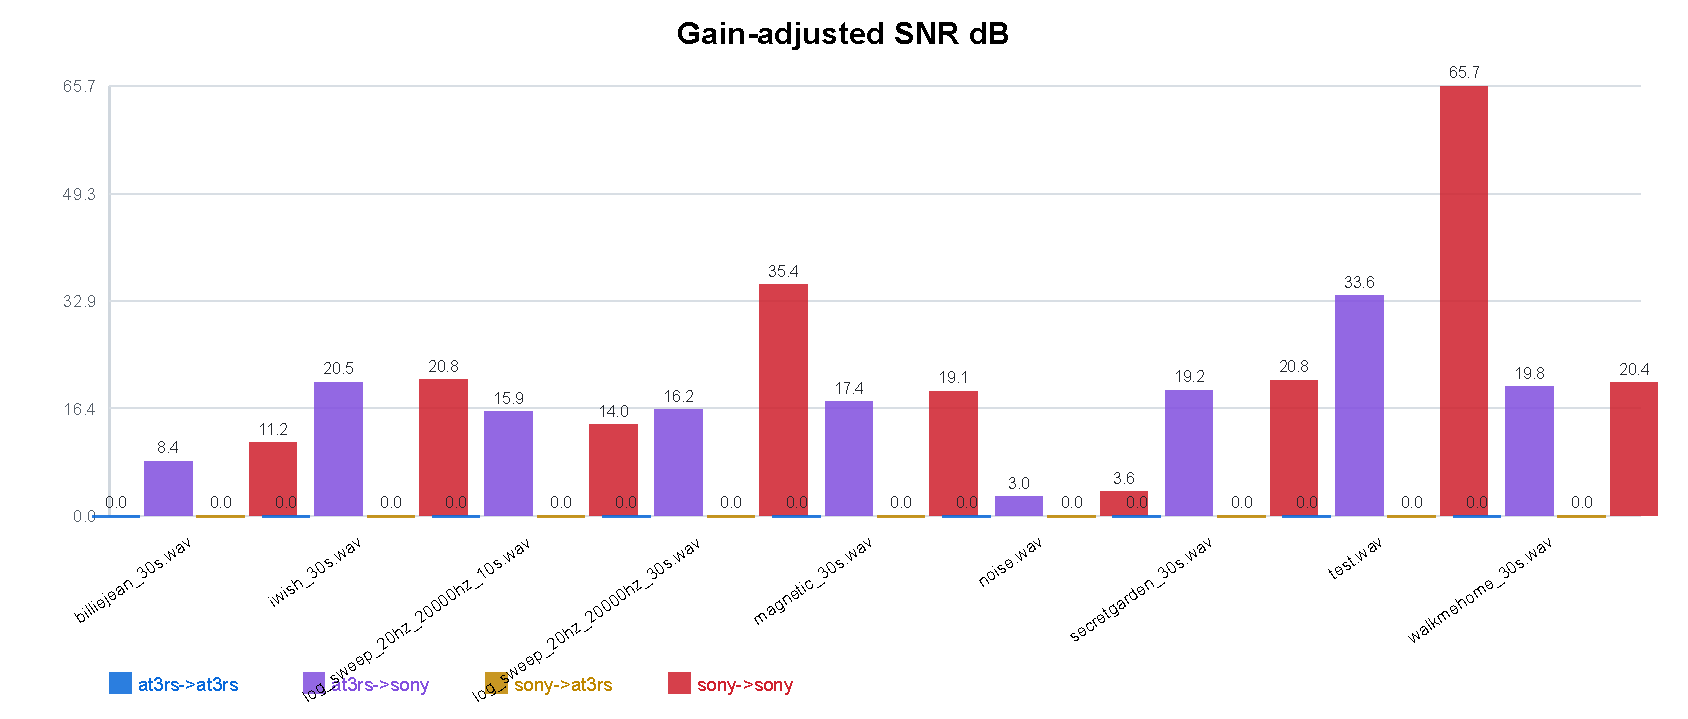
\includegraphics[width=\linewidth]{figures/current_gainadjusted_snr_db.pdf}
\caption{Current gain-adjusted SNR by fixture and encoder/decoder cell. The
gain-adjusted score compensates for scalar output-level differences before
computing residual energy.}
\label{fig:current-gain-snr}
\end{figure}

\begin{figure}[t]
\centering
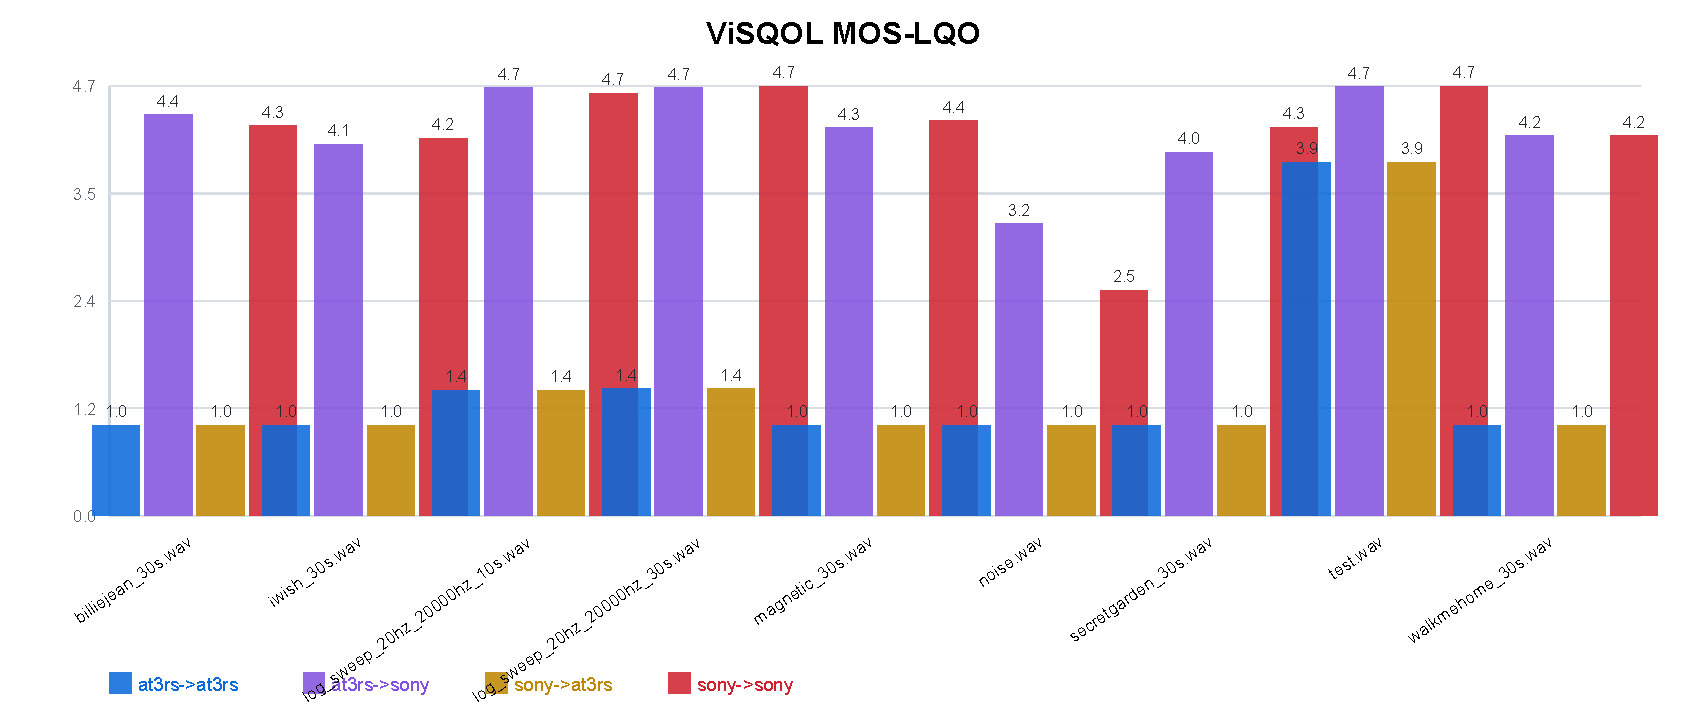
\includegraphics[width=\linewidth]{figures/current_visqol_moslqo.pdf}
\caption{Current ViSQOL MOS-LQO by fixture and encoder/decoder cell. Higher
scores are better; this metric is useful for trend tracking but does not
fully capture crackle, ringing, or pitch-related artifacts.}
\label{fig:current-visqol}
\end{figure}

\begin{figure}[t]
\centering
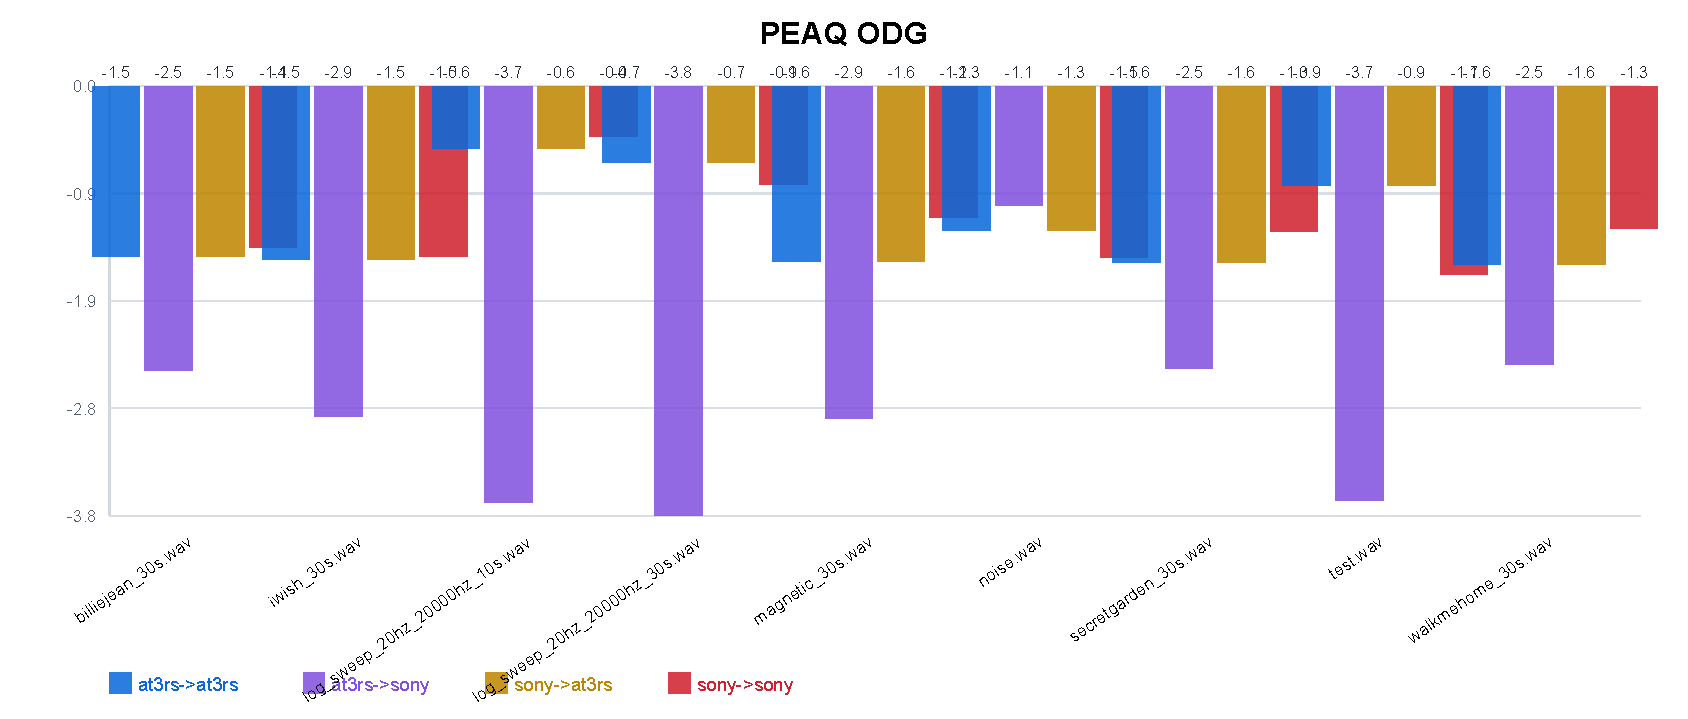
\includegraphics[width=\linewidth]{figures/current_peaq_odg.pdf}
\caption{Current PEAQ ODG by fixture and encoder/decoder cell. ODG ranges
from \(0\) for imperceptible impairment toward \(-4\) for very annoying
impairment; higher is better.}
\label{fig:current-peaq}
\end{figure}

\section{Implementation Notes and Limitations}
\label{sec:limitations}

\paragraph{Decoder.} The \texttt{-d} path parses RIFF/WAVE ATRAC3 files with
format tag \(0\text{x}0270\), extracts frame payloads using the container block
alignment, and writes PCM WAV output. It is kept wired into the CLI and eval
runner so decoder progress can be measured, but current decoded PCM is not
usable quality: recent matrix runs show the at3rs-decoder cells near
\(0\,\text{dB}\) SNR while Sony decoding of the same at3rs bitstream scores
much higher. Decoder correctness is therefore a separate open problem, not
evidence that the at3rs encoder bitstream is undecodable.

\paragraph{Sampling rates.} Only \(44.1\,\text{kHz}\) input is supported.
The QMF prototype filter and the loudness/ATH curves are tabulated for
this rate; supporting \(48\,\text{kHz}\) or \(32\,\text{kHz}\) ATRAC3
variants would require regenerating these tables.

\paragraph{Tuning.} The constants in
Eq.~\ref{eq:masking}--\ref{eq:initial_selector}
(\(0.98\), \(0.01\), \(\Lambda_{\text{factor}}\), the importance and
shape-hint vectors, the divisor steps in
\texttt{selector\_spread\_divisor}) are fitted to the payload fixtures
and are not derived from a principled rate-distortion optimisation. The
shape of the bit-allocation pipeline mirrors FFmpeg's encoder
\texttt{atrac3enc.c} but the exact numeric tradeoffs differ.

\paragraph{ATRAC3+.} \texttt{src/atrac3plus\_data.rs} contains the lookup
tables (\texttt{ATRAC3P\_WL\_CBS}, \texttt{ATRAC3P\_CT\_CBS},
\texttt{ATRAC3P\_SPECTRA\_CBS}, etc.) needed by the wider ATRAC3+
toolchain, but no ATRAC3+ encoding or decoding is implemented in this
workbench. They are reserved for a future companion module.

\section*{Acknowledgements}

This workbench builds on prior reverse-engineering work on
\textsc{atrac3} that is reflected in the FFmpeg source tree
(\texttt{libavcodec/atrac3*.c}). The QMF prototype filter coefficients
and the seven Huffman tables in this document are reproductions of those
artefacts.

\appendix
\section{Reference Constant Map}
\label{app:constants}

\begin{table}[ht]
\centering\small
\begin{tabular}{lll}
\toprule
Symbol & Value / source & Location \\
\midrule
\(F_s\) & \(44{,}100\,\text{Hz}\) & required \\
\(N\)   & \(1024\) samples/frame  & \texttt{atrac3.rs} \\
\(B_{\text{ch}}\) & \(96/152/192\,\text{B}\) & \texttt{main.rs:153} \\
\(h_{\text{half}}\) & \(24\)-tap & \texttt{atrac3.rs:16} \\
\(\sigma[k]\) & \(2^{k/3 - 21}\) & \texttt{atrac3.rs:36} \\
\(w_a\) & Eq.~\ref{eq:enc_window} & \texttt{atrac3.rs:54} \\
\(w_s\) & Eq.~\ref{eq:dec_window} & \texttt{atrac3.rs:62} \\
\(\mathcal{L}\) & loudness curve & \texttt{atrac3.rs:72} \\
\(T_{\text{ATH}}\) & per-BFU ATH & \texttt{atrac3.rs:83} \\
\(\Lambda_{\text{factor}}\) & \(0.006\) & \texttt{atrac3.rs:122} \\
\(\phi_b\) & fixed alloc & \texttt{atrac3.rs:107} \\
\(\gamma_b^{(S)}\) & shape hint & \texttt{atrac3.rs:113} \\
\bottomrule
\end{tabular}
\caption{Map from symbols used in this document to their definitions in
the source tree.}
\label{tab:constants}
\end{table}

\end{document}
